\documentclass[12pt,a4paper]{article}
\usepackage[utf8]{inputenc}
\usepackage[spanish]{babel}
\usepackage{amsmath}
\usepackage{amsfonts}
\usepackage{amssymb}
\usepackage{graphicx}
\usepackage{kpfonts}
\usepackage[left=2cm,right=2cm,top=2cm,bottom=2cm]{geometry}
\title{EV 1-6 OPERACIÓN DE CIRCUITOS DE ACTIVACIÓN CON TIRISTORES EN CONVERTIDORES DE CA-CD y CA-CA}
\author{Giovanni Daniel Ruiz Tinoco\\
\small Sistemas electrónicos de interfaz\\
  \small Universidad Politécnica de la zona metropolitana de Guadalajara\\
  \small 4-B \\
  \small Ing. Mecatrónica\\
\centering

\includegraphics[scale=2]{imagenes/upz.jpg} 
}

\begin{document}
\maketitle
\newpage
\begin{center}
\section {Tiristores}
\end{center}
Vamos a comenzar con lo que es un tiristor, un tiristor es un semiconductor de potencia que se utiliza como interruptor, ya sea para conducir o interrumpir la corriente eléctrica, a este componente se le conoce como de potencia por que se utilizan para manejar grandes cantidades de corriente y voltaje, a comparación de los otros semiconductores que manejan cantidades relativamente bajas.\\
Cuando se habla de tiristores comúnmente se cataloga al tiristor como un SRC (silicon controlled rectifier), pero esto no es del todo correcto ya que este tipo es el más popular y conocido pero no es el único que existe.\\
\begin{center}
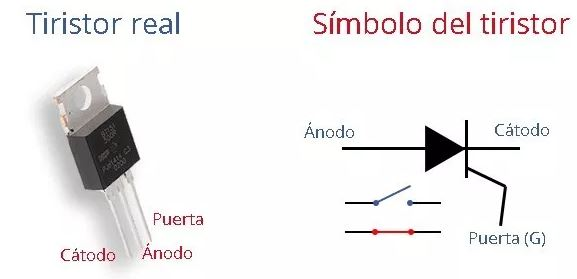
\includegraphics[scale=1]{imagenes/tiristor.JPG} 
\subsection{¿Cómo funciona un tiristor?}
\end{center}
\begin{flushleft}
Los tiristores están conformados por 3 terminales un ánodo, un cátodo y una compuerta o mejor conocida “gate”, su funcionamiento se asemeja al de un relevador o un interruptor mecánico, Ya que cuando aplicas una corriente a la terminal gate este se activa y obtiene la característica de dejar pasar a la electricidad.\\
\end{flushleft}
\begin{center}
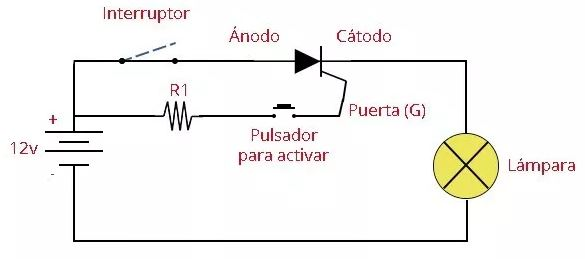
\includegraphics[scale=0.8]{imagenes/tiristor2.JPG} 
\end{center}
\newpage
\begin{center}
\section {Tiristores en CA}
\end{center}
La mayoría de las aplicaciones de los tiristores o/y los SCR son para controlar un circuito de alimentación o salida en corriente alterna (interruptor). Como ya dijimos, el tiristor solo conduce si está polarizado directamente, es decir si el ánodo está al polo positivo y el cátodo al negativo.\\ Pues bien ¿Qué pasaría si la tensión de alimentación y activación fuera la misma y en corriente alterna? \\
\begin{center}
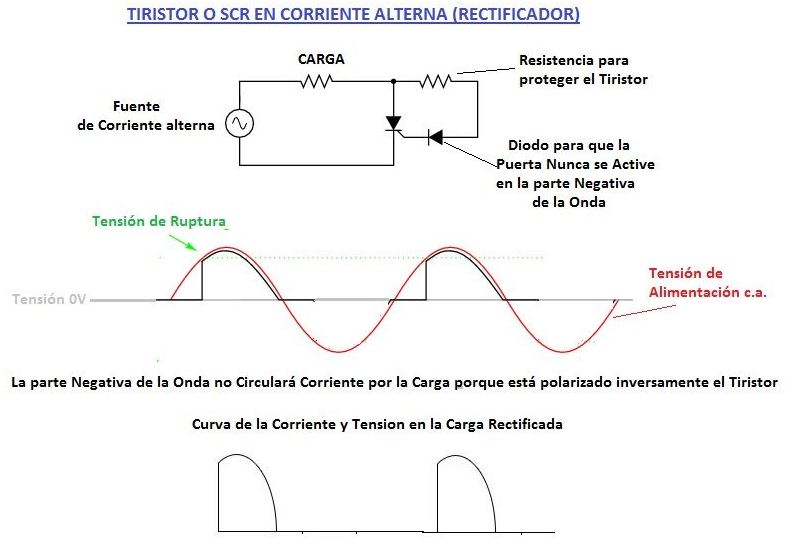
\includegraphics[scale=0.8]{imagenes/tiristorCA.JPG} 
\end{center}
\begin{flushleft}
Durante el semiciclo positivo de la fuente de corriente alterna (c.a.) el ánodo del tiristor o SCR es mas positivo que el cátodo y están polarizados directamente. Si ahora le llega una señal suficiente a la puerta el tiristor se activará y pasará corriente de entre ánodo y cátodo. Al principio del ciclo positivo de la onda como no le llega la suficiente corriente a la puerta el tiristor estará desactivado. Llegará un momento que le llegue la suficiente corriente o tensión (tensión de disparo) y es entonces cuando el tiristor se activará por lo tanto una parte de la onda no estará en la salida al principio.\linebreak

Al pasar por cero, mejor dicho por el valor de la corriente de mantenimiento IK, el tiristor se desconecta (sin corriente de salida = interruptor abierto). Durante el otro medio ciclo la polaridad de la fuente es negativa, y esta polaridad hace que el tiristor o SCR quede inversamente polarizado lo cual impide que circule cualquier corriente hacia la carga. Esto significa que no puede estar en conducción por más de medio ciclo. Al volver al ciclo positivo necesitamos activar de nuevo el tiristor con una pequeña corriente en la puerta, pero como está conectada también a la fuente de tensión en alterna, la propia fuente nos la genera.\\
\end{flushleft}
\newpage
\begin{flushleft}
Pues resulta que en la parte de la onda positiva de corriente alterna circula corriente y por la parte negativa no circula corriente, haciendo el tiristor de rectificador, ya que la onda de salida quedaría rectificada (solo la parte positiva).\linebreak

Para evitar que a la puerta le llegue corriente inversa, podemos hacer el circuito de activación a través de un sencillo diodo simple, para que entrega corriente a la puerta G solo en una dirección y además esta corriente estará un poco desfasada con respecto a la de salida por culpa del receptor o resistencia de salida. Si no colocamos el diodo puede que el tiristor se active con una tensión inversa y esto no debe ocurrir. Fíjate que en la curva característica del tiristor de la figura de arriba también hay una pequeña corriente inversa, de la que no hablamos.\linebreak

El tiristor así usado es realmente al que se conoce como SCR. hay unos tiristores especiales que son capaces de conducir en los dos sentidos (bidireccionales) y en este tipo la onda de salida o carga en corriente alterna tendría una componente positiva y también otra cuando la onda es negativa. Estos tiristores se llaman "TRIAC" (puedes saber más sobre ellos en el enlace). De estos últimos también haremos un estudio a parte.
\end{flushleft}
\newpage

\begin{center}
\section{Tiristores en CD}
\subsection{Activacion del tiristor (SCR) en corriente contínua}
\end{center}
\begin{flushleft}
En el gráfico se ve una aplicación sencilla del tiristor en corriente continua. El tiristor se comporta como un circuito abierto hasta que activa su compuerta (GATE) con un pulso de tensión que causa una pequeña corriente. (se cierra momentáneamente el interruptor S). El tiristor conduce y se mantiene conduciendo, no necesitando de ninguna señal adicional para mantener la conducción. No es posible desactivar el tiristor (que deje de conducir) con la compuerta.\\
\end{flushleft}
\begin{center}
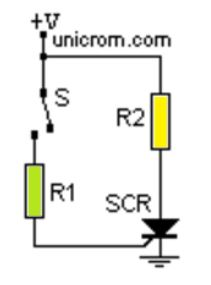
\includegraphics[scale=1]{imagenes/tiristorCD.JPG} 
\subsection{Características del pulso de disparo}
\end{center}
\begin{flushleft}La duración del pulso aplicado a la compuerta G debe ser lo suficientemente largo para asegurar que la corriente de ánodo se eleve hasta el valor de retención. Otro aspecto importante a tomar en cuenta es la amplitud del pulso, que influye en la duración de éste.\newline
\end{flushleft}
\begin{center}
\subsection{Desactivación de un tiristor}
\end{center}
El tiristor una vez activado, se mantiene conduciendo, mientras la corriente de ánodo (IA) sea mayor que la corriente de mantenimiento (IH). Normalmente la compuerta (G) no tiene control sobre el tiristor una vez que este está conduciendo.
\newpage
\begin{center}
\subsection{Opciones para desactivar un tiristor:}
\end{center}
\begin{flushleft}
—Se abre el circuito del ánodo (corriente IA = 0)

—Se polariza inversamente el circuito ánodo-cátodo (el cátodo tendrá un nivel de tensión mayor que el del ánodo)

—Se deriva la corriente del ánodo IA , de manera que esta corriente se reduzca y sea menor a la corriente de mantenimiento IH.\linebreak

Si se disminuye lentamente el voltaje (tensión), el tiristor seguirá conduciendo hasta que por él una cantidad de corriente menor a la llamada “corriente de mantenimiento o de retención (IH)”, lo que causará que el tiristor deje de conducir aunque la tensión VG (voltaje de la compuerta con respecto a tierra) no sea cero. Como se puede ver el SCR , tiene dos estados:\linebreak

1- Estado de conducción, en donde la resistencia entre ánodo y cátodo es muy baja.\\
2- Estado de corte, donde la resistencia es muy elevada.\\
\end{flushleft}

\end{document}

\section{se}